\documentclass{article}
\usepackage{graphicx} % Required for inserting images

\title{Test OverleafSync}
\author{IWH Macro department}
\date{\today}

\begin{document}

\maketitle

\section{Introduction}

\begin{itemize} 
    \item A warm welcome to today's workshop!
    \item I hope to learn about Git and Overleaf with you!
    \item As you will see, both tools can be combined in a powerful way for collaborative writing!
    \item It is great to work with you
    \item I really look forward
\end{itemize}

\section{Playgrounds}
In the following, everyone will be given the opportunity to add some words to their assigned paragraph in the local copy, and then push the changes to the common document.

\subsection{Playground 1: Katja}

\subsection{Playground 2: Julian}

\subsection{Playground 3: Anna}

\subsection{Playground 4: Oliver}

\subsection{Playground 5: Andrej}

\subsection{Playground 6: Hua}

\subsection{Playground 7: Afroza}

\subsection{Playground 8}

\subsection{Playground 9}
Nice to see you!
\subsection{Playground 10}




\section{Conflict provocation}
Conflicts may arise when working with colleagues on one common project. The following section contains five paragraphs, which the participants will be asked to change simultaneously in order to provoke conflicts!

\subsection{Conflict 1}
Economics is an awesome and beautiful discipline that helps us understand resource allocation and market operations. The IWH has significantly contributed through studies on the economic effects of structural change in Eastern Germany, offering valuable insights for similar regions.

\subsection{Conflict 2}
Economics informs public policy by analyzing data and developing models. IWH researchers have influenced policy debates on labor market reforms and fiscal federalism, helping shape policies that promote economic growth and social welfare.

\subsection{Conflict 3}
Addressing global challenges like poverty and climate change, economics offers evidence-based recommendations. The IWH's research on climate change economics emphasizes the benefits of sustainable development and the need for international cooperation.

\subsection{Conflict 4}
Economics is interdisciplinary, incorporating insights from psychology and sociology to understand human behavior. The IWH fosters collaboration between economists and other experts, leading to innovative research on social networks and cultural factors.

\subsection{Conflict 5}
As a field that is exposed to technological change, economics continually evolves to address new challenges. The IWH pioneers research on the digital economy and technological change, providing insights into taking advantage of digitalization benefits while mitigating risks.

% \newpage
% \section{A nice picture}
% \subsection{I try to add a figure}
% \begin{figure}[h]
%   \centering
%   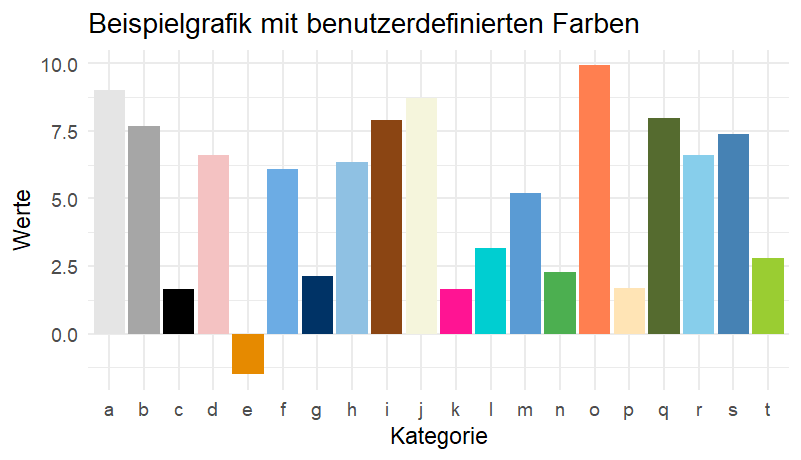
\includegraphics[width=\textwidth]{Figures/efn/plot_example.png}
%   \caption{Caption}
% \end{figure}

\end{document}
